\documentclass[12pt,spanish,openany,letterpaper,pagesize]{scrbook}
\usepackage[utf8]{inputenc}
\usepackage[spanish]{babel}%escribir con acentos sin necesidad de comandos \'{} .
\usepackage{fancyhdr}
%\usepackage{epsfig}
\usepackage{epic}
\usepackage{eepic}
\usepackage{amsmath, amssymb, amsthm, latexsym, graphics, graphpap, layout, wasysym, multicol, enumerate,amsfonts,mathrsfs}
\usepackage{graphics,lscape}
\usepackage[mathscr]{euscript}
\usepackage{xcolor}
\usepackage{verbatim}
\usepackage{booktabs}
\usepackage{float}
\usepackage{hyperref}
\usepackage{threeparttable}
\usepackage{amscd}
\usepackage{here}
\usepackage[pdftex]{graphicx}
\usepackage{lscape}
\usepackage{tabularx}
\usepackage{subfigure}
\usepackage{longtable}
\usepackage{geometry}
\usepackage{cite}
\usepackage{algorithmic}
\usepackage{diagbox}
\usepackage{array,multirow}
\usepackage[all]{ xy}

\usepackage{rotating} %Para rotar texto, objetos y tablas seite. No se ve en DVI solo en PS. Seite 328 Hundebuch
                        %se usa junto con \rotate, \sidewidestable ....

\renewcommand{\theequation}{\thechapter-\arabic{equation}}
\renewcommand{\thefigure}{\textbf{\thechapter-\arabic{figure}}}
\renewcommand{\thetable}{\textbf{\thechapter-\arabic{table}}}

\pagestyle{fancyplain}%\addtolength{\headwidth}{\marginparwidth}
\textheight22.5cm \topmargin0cm \textwidth16.5cm
\oddsidemargin0.5cm \evensidemargin-0.5cm%
\renewcommand{\chaptermark}[1]{\markboth{\thechapter\; #1}{}}
\renewcommand{\sectionmark}[1]{\markright{\thesection\; #1}}
\lhead[\fancyplain{}{\thepage}]{\fancyplain{}{\rightmark}}
\rhead[\fancyplain{}{\leftmark}]{\fancyplain{}{\thepage}}
\fancyfoot{}
\thispagestyle{fancy}%

\addtolength{\headwidth}{0cm}
\unitlength1mm %Define la unidad LE para Figuras
%\mathindent0cm %Define la distancia de las formulas al texto,  fleqn las %descentra
\marginparwidth0cm
\parindent0cm %Define la distancia de la primera linea de un parrafo a la margen

%Para tablas,  redefine el backslash en tablas donde se define la posici\'{o}n del texto en las
%casillas (con \centering \raggedright o \raggedleft)
\newcommand{\PreserveBackslash}[1]{\let\temp=\\#1\let\\=\temp}
\let\PBS=\PreserveBackslash

%Espacio entre lineas
\renewcommand{\baselinestretch}{1.1}

%Neuer Befehl f\"{u}r die Tabelle Eigenschaften der Aktivkohlen
\newcommand{\arr}[1]{\raisebox{1.5ex}[0cm][0cm]{#1}}

%Neue Kommandos
\usepackage{Befehle}
%Inicio del documento. Tener en cuenta que hay archivos auxiliares

\newtheorem{teor}{Teorema}[section]
\theoremstyle{definition}
\newtheorem{definition}[teor]{Definición}
\theoremstyle{example}
\newtheorem{example}[teor]{Ejemplo}
\newtheorem{lema}[teor]{Lema}
\newtheorem{afirmacion}[teor]{Afirmación}
\newtheorem{proposicion}[teor]{Proposición}
\newtheorem{coro}[teor]{Corolario}
\newtheorem{ole}[teor]{Conjetura}
%\theoremstyle{proposicion}

%\def\proof{\paragraph{Demostración:\\}}%\begin{proof}
%\def\endproof{\hfill$\blacksquare$}%\end{proof}

\begin{document}
\pagenumbering{roman}
%\newpage
%\setcounter{page}{1}
\begin{center}
\begin{figure}
\centering%

\includegraphics[scale=0.4]{Imagenes/logo_1.png}
%{file=uc.jpg,scale=1}%
\end{figure}
\thispagestyle{empty} \vspace*{2.0cm} \textbf{\huge
Predicción del comportamiento de una enfermedad simulada en autómatas celulares con un algoritmo propuesto en redes neuronales}\\[6.0cm]
\Large\textbf{Jorge Andrés Ibáñez Huertas}\\[4.0cm]
\small Universidad Central\\
Departamento de Matemáticas\\
Bogotá, Colombia\\
2021\\
\end{center}

\newpage{\pagestyle{empty}\cleardoublepage}

\newpage
\begin{center}
\thispagestyle{empty} \vspace*{0cm} \textbf{\huge
Predicción del comportamiento de una enfermedad simulada en autómatas celulares con un algoritmo propuesto en redes neuronales}\\[3.5cm]
\Large\textbf{Jorge Andrés Ibáñez Huertas}\\[3.0cm]
\small Trabajo de grado presentado como requisito parcial para optar al
t\'{\i}tulo de:\\
\textbf{Matemático}\\[3.0cm]
Director:\\
Carlos Isaac Zainea\\[3.5cm]
Universidad Central\\
Departamento de Matemáticas\\
Bogotá, Colombia\\
2021\\
\end{center}

\newpage{\pagestyle{empty}\cleardoublepage}

% \newpage
% \thispagestyle{empty} \textbf{}\normalsize
% \\\\\\%
% \textit{"Tan sólo por la educación puede el hombre llegar a ser hombre.\\ El hombre no es más que lo que la educación hace de él"\\
% \textit{Immanuel Kant}}\\[4.0cm]

\begin{flushright}
\begin{minipage}{8cm}
    \noindent
        \small
\end{minipage}
\end{flushright}

\newpage{\pagestyle{empty}\cleardoublepage}

\newpage
\thispagestyle{empty} \textbf{}\normalsize
\\\\\\%
\textbf{\LARGE Agradecimientos}\\

% Agradezco a mis padres Roosvelt Rivera y Angelica Useche por los años de apoyo incondicional en mis años de estudio, además de la profesora Edel María Serrano Iglesias (Q.E.P.D) sin la cuál no hubiera entrado al mundo de las matemáticas.\\
% También agradezco a los profesores que a lo largo de la carrera estuvieron dispuestos a enseñar y guiar con incontable paciencia y dedicación, entre ellos: Xiomara Rojas, Diana Herrera, Diana Pulido, Isaac Zainea, Miguel Pachón, Henry Naranjo, Fabián Sánchez, Nicolás Avilán y mi director de tesis Henry Sánchez.

\newpage{\pagestyle{empty}\cleardoublepage}

\newpage
\textbf{\LARGE Resumen}\\

% En este trabajo se desarrollan los resultados obtenidos en el artículo  de Morales \& Arbieto,  específicamente la distancia $GH^0$ dada en ese manuscrito. Una vez se haya comprendido la fundamentación y  analizado algunas propiedades de dicha métrica, se procederá a estudiar la estabilidad topológica de las dinámicas sobre espacios compactos utilizando en principio la noción de Walters con una métrica $C^0$. Luego, se define y analiza la noción de $GH$-estabilidad  resaltando la relación que existe entre ambas nociones.\\

\textbf{\LARGE Abstract}\\\\

% In this work the results obtained in the article by Morales \& Arbieto are developed, specifically, the distance $ GH^0$ given in the article. Once the foundation is understood and some properties of that metric have been analyzed, we will proceed to study the topological stability of the dynamics on compact spaces using a notion given by Walters with a  $C^0$-metric. After that, will be defined and analyzed the $GH$-stability notion highlighting the relationship between both notions.

\renewcommand{\tablename}{\textbf{Tabla}}
\renewcommand{\figurename}{\textbf{Figura}}
\renewcommand{\listtablename}{Lista de Tablas}
\renewcommand{\listfigurename}{Lista de Figuras}
\renewcommand{\contentsname}{Contenido}

%\newcommand{\clearemptydoublepage}{\newpage{\pagestyle{empty}\cleardoublepage}}
\cleardoublepage
\addcontentsline{toc}{chapter}{Lista de figuras} % para que aparezca en el indice de contenidos
\listoffigures % indice de figuras

%\cleardoublepage
%\addcontentsline{toc}{chapter}{Lista de tablas} % para que aparezca en el indice de contenidos

\tableofcontents %% this produces the table of contents - you might have guessed :-)

%\listoftables % indice de tablas

%\chapter*{Lista de s\'{\i}mbolos}
\addcontentsline{toc}{chapter}{\numberline{}Lista de s\'{\i}mbolos}
Esta secci\'{o}n es opcional, dado que existen disciplinas que no manejan s\'{\i}mbolos y/o abreviaturas.\\

Se incluyen s\'{\i}mbolos generales (con letras latinas y griegas), sub\'{\i}ndices, super\'{\i}ndices y abreviaturas (incluir s\'{o}lo las clases de s\'{\i}mbolos que se utilicen). Cada una de estas listas debe estar ubicada en orden alfab\'{e}tico de acuerdo con la primera letra del s\'{\i}mbolo.
\section*{S\'{\i}mbolos con letras latinas}
 \label{simbolos}
 \renewcommand{\arraystretch}{1.3}
%\begin{longtable}[l]{*{4}{>{$}l<{$}}p{9cm}}
\begin{longtable}[l]{>{$}l<{$}l>{$}l<{$}>{$}l<{$}}
%\begin{tabular}
\textbf{S\'{\i}mbolo}&\textbf{T\'{e}rmino}&\textbf{Unidad SI}&\textbf{Definici\'{o}n}\\[0.5ex]\hline
\endfirsthead%
\textbf{S\'{\i}mbolo}&\textbf{T\'{e}rmino}&\textbf{Unidad SI}&\textbf{Definici\'{o}n}\\[0.5ex]\hline
\endhead%
      A              &\'{A}rea                                   &\text{m}^{2}                         &\int\int dxdy\\%
      A_{\text{BET}} &\'{A}rea interna del s\'{o}lido                &\frac{\text{m}^{2}}{\text{g}}        &\text{ver DIN ISO 9277}\\%
      A_{\text{g}}   &\'{A}rea transversal de la fase gaseosa    &\text{m}^{2}                         &\text{Ec...}\\%
      A_{\text{s}}   &\'{A}rea transversal de la carga a granel  &\text{m}^{2}                         &\text{Ec...}\\%
      a              &Coeficiente                            &1                                    &\text{Ec...}\\%
      a              &Contenido de ceniza                    &1                                    &\frac{m_{\text{ceniza}}}{m_{\text{bm,0}}}\\%
      c              &Contenido de carbono                   &1                                    &\frac{m_{\text{C}}}{m}\\%
      c              &Longitud de la cuerda                  &\text{m}                             &\text{Figura...}\\
      c              &Concentraci\'{o}n de la cantidad de materia&\frac{\text{mol}}{\text{m}^{3}}      &\frac{n}{V}\\%
      D              &Di\'{a}metro                               &\text{m}                             &\\%
      E_{\text{A}}   &Energ\'{\i}a de activaci\'{o}n                  &\frac{\text{kJ}}{\text{mol}}         &\text{Ec....}\\%
      F              &Fracci\'{o}n de materia vol\'{a}til            &1                                    &\text{ver DIN 51720}\\%
      Fr             &N\'{u}mero de Froude                       &1                                    &\frac{\omega^{2}R}{g_{\text{0}}}\\%
      \overrightarrow{g}&Aceleraci\'{o}n de la gravedad          &\frac{\text{m}}{\text{s}^{2}}        &\frac{d^{2}\overrightarrow{r}}{dt^{2}}\\%
      H              &Entalp\'{\i}a                               &\text{J}                             &U+PV\\%
      H_{\text{o}}   &Poder calor\'{\i}fico superior              &\frac{\text{MJ}}{\text{kg}}          &\text{ver DIN 51857}\\%
      h              &Contenido de hidr\'{o}geno                 &1                                    &\frac{m_{\text{H}}}{m}\\%
      K              &Coeficiente de equilibrio              &1                                    &\text{Ec...}\\%
      L              &Longitud                               &\text{m}                             &DF\\%
      L              &Longitud del reactor                   &\text{m}                             &\text{Figura...}\\%
      m              &Masa                                   &\text{kg}                            &DF\\%
      \dot{m}        &Flujo de masa                          &\frac{\text{kg}}{\text{s}}           &\frac{m}{t}\\%
      n              &Velocidad de rotaci\'{o}n                  &\frac{\text{1}}{\text{s}}            &\frac{\omega}{2\pi}\\%
      n              &Cantidad de materia                    &\text{mol}                           &DF\\%
      P              &Presi\'{o}n                                &\text{Pa}                            &\frac{\vec{F}\cdot\vec{n}}{A}\\%
      Q              &Calor                                  &\text{kJ}                            &\text{1. $LT$}\\%
      T              &Temperatura                            &\text{K}                             &DF\\%
      t              &Tiempo                                 &\text{s}                             &DF\\%
      x_{\text{i}}   &Fracci\'{o}n de la cantidad de materia     &1                                    &\frac{n_{\text{i}}}{n}\\%
      V              &Volumen                                &\text{m}^{3}                         &\int{dr^{3}}\\%
      \vec{u}        &Velocidad                              &\frac{\text{m}}{\text{s}}            &(\frac{dr}{dt},r\frac{d\upsilon}{dt},\frac{dz}{dt})\\%
      w_{\text{i}}   &Fracci\'{o}n en masa del componente i      &1                                    &\frac{m_{\text{i}}}{m_{\text{0}}}\\%
      w_{\text{w,i}} &Contenido de humedad de la sustancia i &1                                    &\frac{m_{\text{\wasser}}}{m_{\text{i,0}}}\\%
      Z              &Factor de gases reales                 &1                                    &\frac{pv}{RT}\\%
\end{longtable}
\vspace{5ex}
\section*{S\'{\i}mbolos con letras griegas}

\begin{longtable}[l]{>{$}l<{$}l>{$}l<{$}>{$}l<{$}}
\textbf{S\'{\i}mbolo}&\textbf{T\'{e}rmino}&\textbf{Unidad SI}&\textbf{Definici\'{o}n}\\[0.5ex] \hline%
\endfirsthead%
\textbf{S\'{\i}mbolo}&\textbf{T\'{e}rmino}&\textbf{Unidad SI}&\textbf{Definici\'{o}n}\\[0.5ex] \hline%
\endhead%
\renewcommand{\arraystretch}{1.3}
 \label{simbolosg}
     \alpha_{\text{BET}}  &Factor de superficie                  &\frac{\text{m}^{2}}{\text{g}}   &(w_{\text{F,waf}})(A_{\text{BET}})\\%
     \beta_{\text{i}}     &Grado de formaci\'{o}n del componente i   &1                               &\frac{m_{\text{i}}}{m_{\text{bm,0}}}\\%
     \gamma               &Wandhaftreibwinkel (Stahlblech)       &1                               &\text{Secci\'{o}n...}\\
     \epsilon             &Porosidad de la part\'{\i}cula             &1                               &1-\frac{\rho_{\text{s}}}{\rho_{\text{w}}}\\%
     \eta                 &mittlere Bettneigungswinkel (St\"{u}rzen) &1                               &\text{Figura...}\\%
     \theta               &\'{A}ngulo de inclinaci\'{o}n de la cama      &1                               &\text{Figura...}\\
     \theta_{\text{O}}    &\'{A}ngulo superior de avalancha          &1                               &\text{Figura...}\\
     \theta_{\text{U}}    &\'{A}ngulo inferior de avalancha          &1                               &\text{Figura...}\\
     \kappa               &Velocidad de calentamientoe           &\frac{\text{K}}{\text{s}}       &\frac{dT}{dt}\\%
     \nu                  &Coeficiente estequiom\'{e}trico           &1                               &\text{ver DIN 13345}\\%
     \rho_{\text{b}}      &Densidad a granel                     &\frac{\text{kg}}{\text{m}^{3}}  &\frac{m_{\text{S}}}{V_{\text{S}}}\;(\text{Secci\'{o}n...})\\
     \rho_{\text{s}}      &Densidad aparente                     &\frac{\text{kg}}{\text{m}^{3}}  &\frac{m_{\text{F}}}{V_{\text{P}}}\;(\text{Secci\'{o}n...})\\
     \rho_{\text{w}}      &Densidad verdadera                    &\frac{\text{kg}}{\text{m}^{3}}  &\frac{m_{\text{F}}}{V_{\text{F}}}\;(\text{Secci\'{o}n...})\\
     \tau                 &Tiempo adimensional                   &1                               &\text{Ec....}\\%
     \Phi_{\text{V}}      &Flujo volum\'{e}trico                     &\frac{\text{m}^{3}}{\text{s}}   &\frac{\Delta V}{\Delta t}\\
     \omega               &Velocidad angular                     &\frac{1}{\text{s}}              &\frac{d\upsilon}{dt}\\

\end{longtable}


\section*{Sub\'{\i}ndices}
\begin{longtable}[l]{>{}l<{}l}
  \textbf{Sub\'{\i}ndice} & \textbf{T\'{e}rmino} \\[0.5ex] \hline%
  \endfirsthead%
  \textbf{Sub\'{\i}ndice} & \textbf{T\'{e}rmino} \\[0.5ex] \hline%
  \endhead%
\renewcommand{\arraystretch}{1.4}\label{simbolosg}

 bm&materia org\'{a}nica\\%
 DR&Dubinin-Radushkevich\\%
 E&Experimental\\%
 g&Fase gaseosa\\%
 k&Condensado\\%
 Ma&Macroporos\\%
 P&Part\'{\i}cula\\%
 p&Poro\\%
 p&Pirolizado\\%
 R&Reacci\'{o}n\\%
 t&Total\\%
 wf&Libre de agua\\%
 waf&Libre de agua y de ceniza\\%
 0&Estado de referencia\\%

\end{longtable}


\setlength{\extrarowheight}{0pt}


\section*{Super\'{\i}ndices}
\begin{longtable}[l]{>{}l<{}l}
  \textbf{Super\'{\i}ndice} & \textbf{T\'{e}rmino} \\[0.5ex] \hline%
  \endfirsthead%
  \textbf{Super\'{\i}ndice} & \textbf{T\'{e}rmino} \\[0.5ex] \hline%
  \endhead%
\renewcommand{\arraystretch}{1.4}\label{simbolosg}

 n &Coeficiente x\\%



\end{longtable}


\setlength{\extrarowheight}{0pt}


\section*{Abreviaturas}
\begin{longtable}[l]{>{}l<{}l}
  \textbf{Abreviatura} & \textbf{T\'{e}rmino} \\[0.5ex] \hline%
  \endfirsthead%
  \textbf{Abreviatura} & \textbf{T\'{e}rmino} \\[0.5ex] \hline%
  \endhead%
\renewcommand{\arraystretch}{1.4}\label{simbolosg}
 1.$LT$&Primera ley de la termodin\'{a}mica\\%
 $DF$    &Dimensi\'{o}n fundamental\\%
 $RFF$   &Racimos de fruta fresca\\%

\end{longtable}


\setlength{\extrarowheight}{0pt}
%\include{Resumen}%\newcommand{\clearemptydoublepage}{\newpage{\pagestyle{empty}\cleardoublepage}}

\pagenumbering{arabic}
\include{Contenidos/C1-Epidemiología}
\chapter{Modelos clásicos}
\section{El modelo SIS}

Analizaremos uno de los casos más generales del modelo SIS, el modelo en el que se consideran las muertas causadas por la enfermedad junto con la natalidad y mortalidad de la población. En este modelo se consideran 2 posibles estados, susceptibles (S) e infectados (I).

Las variaciones entre estados vienen dadas por los nuevos contagios y los individuos que se recuperan de la enfermedad, adicionalmente cada estado se ve afectado por los parámetros que describen la natalidad/mortalidad y la muerte a cauda de la enfermedad. Los diferentes estados del modelo se pueden apreciar en el siguiente diagrama:

\begin{figure}[h]
  \centering
    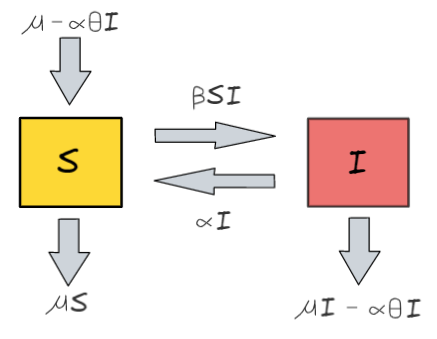
\includegraphics[width=0.4\textwidth]{Imagenes/SIS_compartimientos.PNG}
  \caption{Diagrama de compartimientos para el modelo SIS}
  \label{fig:ClasicSIS}
\end{figure}

En nuestro caso consideraremos una población de tamaño constante y normalizado, por lo que $S + I = 1$ y en consecuencia $S' + I' = 0$.

Típicamente cuando se habla de modelos epidemiológicos con muerte por enfermedad se consideran 4 parámetros: la tasa de infección $\beta$ que representa la probabilidad que tiene un individuo susceptible de adquirir la enfermedad luego de un contagio con un infectado, la tasa de recuperación $\alpha$ que se puede entender como la probabilidad de que un infectado se recupere de la enfermedad, la tasa de natalidad/mortalidad $\mu$ que en el caso de los modelos clásicos se considera igual y finalmente la tasa de muerte por enfermedad $\theta$.

Podemos describir el modelo a partir de un sistema de ecuaciones diferenciales como sigue:

\begin{equation}
\left\{
\begin{array}{l}
S' = \mu(1 - S) + (1 - \theta)\alpha I - \beta S I \\
I' = \beta S I - (1 - \theta)\alpha I - \mu I
\end{array}
\right.
\end{equation}

A continuación determinaremos en que escenarios una enfermedad sería endémica, para esto debemos calcular el valor de $R_0$ correspondiente a nuestro sistema de ecuaciones diferenciales.

Podemos apreciar que los nuevos infectados vienen dados por el término $\beta S$, además como para determinar el valor de $R_0$ se debe suponer una población completamente susceptible tenemos que $b(t) = \beta$. Por otro lado, los flujos que determinan la salida del estado de infección de los individuos viene dado por los términos $-\alpha(1-\theta)I-\mu I$, con lo que si llamamos $I(t)$ a la cantidad de individuos infectados que permanecieron infectados desde el momento 0, tenemos

\begin{equation}
\frac{dI}{dt} = -\alpha(1-\theta)I-\mu I
\end{equation}

Donde al usar el método de separación de variables obtenemos

\begin{equation}
I(t) = I(0)e^{-(\alpha(1-\theta)+\mu)t}
\end{equation}

De ese modo podemos afirmar que la proporción de individuos que permanecen infectados hasta un tiempo $t$ viene dado por $e^{-(\alpha(1-\theta)+\mu)t}$, con lo cual $F(t)=e^{-(\alpha(1-\theta)+\mu)t}$.

Finalmente, para determinar el valor de $R_0$ debemos calcular:

\begin{align}
R_0 &= \lim_{T\to\infty}\int_0^T b(t)F(t) dt \\
&= \lim_{T\to\infty}\int_0^T \beta e^{-(\alpha(1-\theta)+\mu)t} dt\\
&= \frac{\beta}{\alpha(1-\theta)+\mu}
\end{align}

$\textbf{Observación:}$ La ecuación $I(t)$ nos permite afirmar que la cantidad de individuos infectados tiende a cero cuando $t$ tiende a infinito.

Analicemos ahora la estabilidad de nuestro modelo SIS, para esto debemos reconocer los puntos en de equilibrio de nuestro sistema de ecuaciones diferenciales. Los puntos están dados por $P_0=(S_a,I_a)=(1,0)$ y uno en $P_1=(S_b,I_b)=\left(\frac{\alpha(1-\theta)+\mu}{\beta},\frac{\beta-\alpha(1-\theta)-\mu}{\beta}\right)$.

A continuación verificaremos que los puntos críticos efectivamente satisfacen las condiciones de ser positivos y menores o iguales a 1:

En el caso de $P_0$ la verificación es trivial. Por otro lado para el caso de $P_1$ observe que 

$$0\leq\alpha(1-\theta)+\mu\leq\beta \longrightarrow \frac{\alpha(1-\theta)+\mu}{\beta}\text{, }\frac{\beta+\alpha(1-\theta)+\mu}{\beta}\geq0$$

Si dividimos la expresión del lado izquierdo por $\beta$ obtenemos

$$0\leq \frac{\alpha(1-\theta)+\mu}{\beta}\leq1$$

De donde podemos afirmar que 

$$1-\frac{\alpha(1-\theta)+\mu}{\beta}\leq1 \longrightarrow \frac{\beta-\alpha(1-\theta)-\mu}{\beta}\leq1$$

De ese modo concluimos que ambos puntos de equilibrio cumplen las condiciones de tener coordenadas positivas y menores que la unidad.

Es momento de determinar los comportamientos que describen ambos puntos, $P_0$ y $P_1$. Para esto consideremos el jacobiano de nuestro modelo dado por:

$$|A-\lambda I|=
\left|\begin{array}{cc}
-\mu-\beta I-\lambda & \lambda(1-\theta)-\beta S \\
\beta I & \beta S-\alpha(1-\theta)-\mu-\lambda
\end{array}\right|$$

Si evaluamos en $P_0$ obtendremos los valores propios

$$\left\{\begin{array}{l}\lambda=-\mu \\
\lambda=\beta-\alpha(1-\theta)-\mu\end{array}\right.$$

Con lo cual, podemos afirmar que si $R_0>1$, $P_0$ se comportará como un punto de silla y por otro lado, si $R_0<1$ estaremos ante un nodo estable. Para el caso de $P_1$ tendremos un comportamiento tipo sumidero dado que $\lambda=0,\lambda=-\mu$ son los valores propios asociados a $P_1$.

## Estudio numérico

Para representar las soluciones del sistema de ecuaciones diferenciales que describe el modelo SIS usaremos el método de Euler, el cual se implementó en el módulo: ´´CompartmentalModelsInEDOS´´.

De manera general, dadas unas condiciones iniciales $S(0)=S_0,I(0)=I_0$ aplicamos el método de Euler a partir de la siguiente expresión

$$\left\{\begin{array}{l}
S_{t+1} = S_t + h\cdot(\mu(1 - S_t) + (1 - \theta)\alpha I_t - \beta S_t I_t ) \\
I_{t+1} = I_t + h\cdot(\beta S_t I_t - (1 - \theta)\alpha I_t - \mu I_t)
\end{array}\right.$$

Discretizaremos el tiempo en días tomando como escala $1\text{ día}=0.1$, es decir, $h=0.1$.

\section{El modelo SIR}

Al igual que en el caso del modelo SIS, nos centraremos en una de las versiones mas generales del modelo SIR en donde se mantenga constante el tamaño de la población.

Para este modelo se considera el estado de inmunidad frente a la enfermedad R. A diferencia del modelo SIS, en el modelo SIR no hay una interacción del estado I al estado S ya que se supone que los individuos que se recuperen de la enfermedad no podran volver a contraerla, por lo que pasaran al estado R. 

En el siguiente diagrama se puden apreciar las interaciones para los estados del modelo:

\begin{figure}[h]
  \centering
    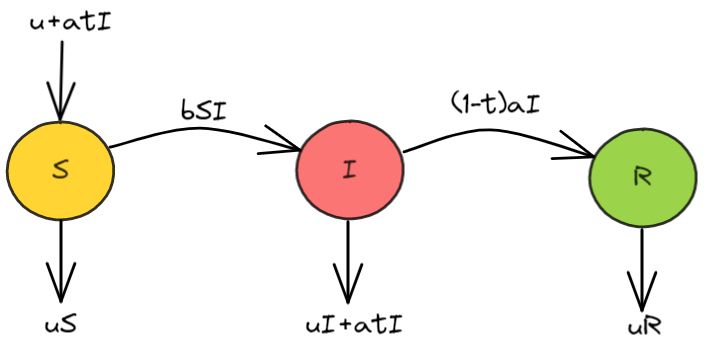
\includegraphics[width=0.6\textwidth]{Imagenes/SIR_compartimientos.PNG}
  \caption{Diagrama de compartimientos para el modelo SIR}
  \label{fig:ClasicSIR}
\end{figure}

De ese modo, el sistema de ecuaciones diferenciales que describe las interacciones entre estados viene dado por la siguiente ecuación:

\begin{equation}
\left\{
\begin{array}{l}
S' = \mu(1 - S) + \alpha\theta I - \beta S I \\
I' = \beta S I - \mu I - \theta\alpha I - (1 - \theta)\alpha I = \beta S I - \alpha I - \mu I \\
R' = \alpha I - \alpha\theta I - \mu R
\end{array}
\right.
\end{equation}

En este caso, la ecuación diferencial que describirá la cantidad de individuos infectados desde el momento 0 viene dada por:

$$\frac{dI}{dt}=-\mu I - \alpha I \longrightarrow I(t)=I(0)e^{-(\alpha+\mu)t}$$

Con lo que $F(t)=e^{-(\alpha+\mu)t}$. La función $b(t)$ estará definida de la misma manera que en el modelo SIS por su naturaleza. De ese modo 

\begin{align}
R_0 &= \int_0^\infty b(t)F(t) dt \\
&= \lim_{T\to\infty} \int_0^T b(t)F(t) dt \\
&= \frac{\beta}{\alpha+\mu}
\end{align}

$\textbf{Observación:}$ Para el modelo SIR la población de infectados tendera a cero cuando $t$ tienda a infinito, debido a la expresión .

A continuación vamos a proceder de la misma manera que en el modelo SIS para analizar la estabilidad de nuestro modelo:

Para nuestro modelo SIR los puntos de equilibrio son:

$$\begin{array}{cc}
P_0=(S_a,I_a,R_a)=(1,0,0) & P_1=(S_b,I_b,R_b)=\left(\frac{\alpha+\mu}{\beta},\frac{\mu(\beta-\alpha-\mu)}{\beta(\mu+(1-\theta)\alpha)},\frac{(1-\theta)\alpha(\beta-\alpha-\mu)}{\beta(\mu+(1-\theta)\alpha)}\right)
\end{array}$$

Veamos que las coordenadas de ambos puntos cumplen las condiciones de ser positivos y menores o iguales que uno: en el caso de $P_0$ se cumple de manera trivial.

Dado que $\alpha,\beta,\theta$ y $\mu$ son valores positivos podemos afirmar que $S_b>0$, para $I_b$ y $R_b$ observe que 

$$\begin{array}{ccc}
\frac{\mu(\beta-\alpha-\mu)}{\beta(\mu+(1-\theta)\alpha)},\frac{(1-\theta)\alpha(\beta-\alpha-\mu)}{\beta(\mu+(1-\theta)\alpha)}>0 & \text{, si} & \beta-\alpha-\mu>0
\end{array}$$

De la ecuación anterior podemos afirmar que 

$$\beta-\alpha-\mu>0\longrightarrow1>\frac{\alpha+\mu}{\beta}$$

además, como ya sabemos que se trata de un valor positivo podemos deducir que 

\begin{align}
1&>1-\frac{\alpha+\mu}{\beta} \\
&= \frac{(\beta-\alpha-\mu)(\mu+(1-\theta)\alpha)}{\beta(\mu+(1-\theta)\alpha)}\\
&= \frac{\mu(\beta-\alpha-\mu)}{\beta(\mu+(1-\theta)\alpha)}+\frac{(1-\theta)\alpha(\beta-\alpha-\mu)}{\beta(\mu+(1-\theta)\alpha)}
\end{align}

Con lo cual,

$$\frac{\mu(\beta-\alpha-\mu)}{\beta(\mu+(1-\theta)\alpha)},\frac{(1-\theta)\alpha(\beta-\alpha-\mu)}{\beta(\mu+(1-\theta)\alpha)}<1$$

Hemos demostrado que ambos puntos de equilibrio cumplen con las condiciones de tener coordenadas positivas y menores a la unidad. Ahora analizaremos la estabilidad de nuestro modelo SIR, para esto usaremos nuevamente el jacobiano de nuestro sistema de ecuaciones diferenciales, esto es

$$|A-\lambda I|=(-\mu-\lambda)
\left|\begin{array}{cc}
-\beta I-\mu-\lambda & -\beta S+\theta\alpha\\
\beta I & \beta S-\alpha-\mu -\lambda
\end{array}\right|$$

Si evaluamos en el punto $P_1$, podemos identificar un comportamiento de tipo silla si $\beta-\alpha-\mu>0$, en caso contrario nos encontraremos ante un nodo estable.

Si tomamos ahora el punto $P_2$ y observamos los valores propios 

$$\left\{\begin{array}{l}
\lambda=-\mu\\
\lambda=-\frac{1}{2}\frac{\mu\beta-\mu\theta\alpha+\sqrt{(\mu\beta-\mu\theta\alpha)^2-4\mu(\beta-\alpha-\mu)(\alpha+\mu-\theta\alpha)^2}}{\alpha+\mu-\theta\alpha} \\
\lambda=-\frac{1}{2}\frac{\mu\beta-\mu\theta\alpha-\sqrt{(\mu\beta-\mu\theta\alpha)^2-4\mu(\beta-\alpha-\mu)(\alpha+\mu-\theta\alpha)^2}}{\alpha+\mu-\theta\alpha}
\end{array}\right.$$

Y de ese modo obtendremos dos tipos de comportamientos, una espiral estable si los valores propios son imaginarios y un nodo estable en el caso de que los valores propios sean reales.
\cite{mateModelsInPopulationAndEpidemiology}
% \chapter{Conclusiones}

% Al realizar este trabajo se comprendió la manera en que se define la distancia $C^0$,\,la distancia de \textit{Hausdorff},\, la distancia \textit{Gromov-Hausdorff}. Así mismo, cómo se pueden calcular distancias entre objetos en donde estas métricas estén definidas usando las diversas caracterizaciones de distancia, así como propiedades que éstas o los objetos (conjuntos, espacios, funciones) poseen. Posterior a eso, fue posible entender qué motiva y cómo funciona la denominada distancia $GH^0$. Ya con estos conceptos claros, se logró comprender de qué manera difieren o son similares ciertos espacios y/o funciones en términos de qué tan cercanos son con respecto a una forma de definir esa distancia. Luego de eso, fue posible a través del entendimiento del concepto de estabilidad topológica de Walters \cite{WalPOTP}, estudiar la propuesta de $GH$-estabilidad topológica dada por Arbieto \& Morales en \cite{AM}.\\

% Las conclusiones que se pueden enunciar de este trabajo son:
% \begin{itemize}
%     % \item Mediante la introducción de métricas o pseudo métricas es posible estudiar y entender el comportamiento de espacios y sistemas, en el sentido de  comparar con elementos cercanos. A su vez, estudiar fenómenos de convergencia y estabilidad.
%     \item Todo homeomorfismo topológicamente estable es isométricamente estable. Sin embargo el recíproco es falso en general.
%     \item Un homeomorfismo topológicamente $GH$-estable es isometricamente estable. Esto quiere decir que una función $GH$-estable ante pequeñas perturbaciones no solo produce una función con una estructura dinámica, sino que además la dinámica misma de la perturbación es muy cercana. 
%     \item Existe un homeomorfismo el cual es topológicamente estable pero no es topológicamente $GH$-estable. Por ende, la $GH$-estabilidad es una condición distinta de estabilidad.
%     \item Todo homeomorfismo topológicamente $GH$-estable en el circulo es topológicamente estable.
%     \item Todo homeomorfismo  expansivo con la P.O.T.P  de un espacio métrico compacto es topológicamente $GH$-estable (extendiendo el resultado dado por Walters).
%     \item Toda función continua positivamente expansiva con la $P.O.T.P_+$ de un espacio métrico compacto es topológicamente $GH-$estable (Caso no invertible).
%     \item Lo desarrollado en este trabajo sugiere que en espacios compactos la $GH$-estabilidad es una condición más fuerte que la estabilidad topológica. Sin embargo, esto aún no ha sido probado.
% \end{itemize}
% \include{Contenidos/Apéndices}

\addcontentsline{toc}{chapter}{\numberline{}Bibliografía}
\bibliographystyle{plain} % apalike
\bibliography{BibliMSc}
\end{document}